%!TEX root = ./../main.tex
\section{Einleitung}\label{sec:Einleitung}
Wikipedia ist eine freie Online-Enzyklopädie, mit dem Ziel „eine frei lizenzierte und hochwertige Enzyklopädie zu schaffen und damit lexikalisches Wissen zu verbreiten“ \cite{wales.}. Sie umfasst 74 Millionen Artikel, die von einer Community von 137.571 Nutzern erstellt und geprüft wurden. Seit 2001 wurden Artikel 877.073.914 mal editiert, dies entspricht etwa 4.000.000 Edits pro Monat. \cite{wikistat}\\

Aufgrund des kollaborativen Erstellungsprozesses können die Nutzer autonom und dynamisch Artikel ändern und erstellen \cite{wikipedia.}.
Die Gründe, weswegen die Nutzer aktiv werden, variieren, einer davon ist die Dokumentation globaler Vorfälle. Dies können politische Veränderungen, Naturkatastrophen, sportliche Ereignisse oder Entwicklungen in der Vita prominenter Personen sein. Eine wichtige Eigenschaft dieser Vorfälle, ist eine hohe Relevanz für einen großen Nutzerkreis. Das führt zu vielen Aktivitäten, sogenannten Edits. Interessant ist dabei auch welche Untermenge sich aus den aktiven Nutzern dafür bildet. Offensichtliche gemeinsame Eigenschaften dieser Nutzermengen sind geographische Verortung, Sprache, Kompetenzen und Interessen. \cite{10.1007978-3-642-36973-5_22}\\

Eine Untersuchung der Aktivitäten der Nutzer über definierte Zeiträume hinweg und mittels statistisch gestützter Analyse kann weitere Zusammenhänge herstellen. Dafür gibt es zwei Herangehensweisen; eine Analyse gespeicherter Aktivitäten, sowie eine Beobachtung in Echtzeit. Georgescu et al. \cite{10.1007978-3-642-36973-5_22} haben in 'Extracting Event-Related Information from Article Updates in Wikipedia' ersteres durchgeführt, worauf im Abschnitt 'Verwandte Arbeiten' eingegangen wird. \\

Für eine Analyse in Echtzeit wird die Folge von Nutzer-Aktivitäten als Stream abgebildet und die Aktivitäten als Events. Wikipedia bietet eine entsprechende Schnittstelle an, den Edit-Events-Stream. Um inhaltliche oder logische Zusammenhänge der Aktivitäten zu erkennen wird im Event-Stream nach Mustern gesucht. Dazu werden in einer Event-Driven-Architecture Operationen auf den Event-Stream angewendet, die unter anderem die Events filtern, aggregieren und gruppieren. Die gewonnenen Zusammenhänge können als Events in den Stream zur weiteren Verarbeitung eingefügt werden, sie können selbst zum Erkennen eines Musters herangezogen werden. Eine stufenweise Verdichtung der Information, mit jeder weiteren Erkennung von Mustern, ist die Folge. Das Resultat sind Zusammenhänge die denen eines Use Case entsprechen.

TODO
    \begin{itemize}
        % \item Für eine Entität (z.\,B. eine Person des öffentlichen Lebens) aus der Gesamtheit der Wikipedia-Edit-Events in "Echtzeit" Events der realen Welt ableiten.
        \item Wir betrachten nur die Metadaten (Zeitstempel, Autor, ...) und nicht den Inhalt der Änderung Änderung (z.\,B. textuelle Änderung).
        \item ...
    \end{itemize}
    Wie sieht so ein Burst of Wikipedia-Edits aus \ref{fig:donald_rumsfelds_resignation_burst}?


\begin{figure}[h]
    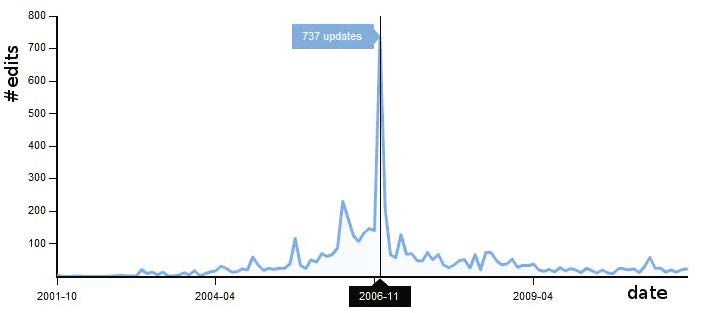
\includegraphics[width=.5\textwidth]{images/Extracting_EventRelated_Information_from_Article.jpg}
    \caption{Donald Rumsfeld’s Rücktritt führte zu einem Burst an Autoren, die einen Wikipedia-Edit vornahmen \cite{10.1007978-3-642-36973-5_22}.}
    \label{fig:donald_rumsfelds_resignation_burst}
\end{figure}